% =============================================================================
% RESULTS - CITA Paper in ALKALI Format
% =============================================================================

\vspace{-2mm}
\section{Results}
\label{sec:results}

We present evaluation results across 5 benchmarks, comparing 6 model variants. We use deterministic metrics following best practices from holistic evaluation~\cite{liang2023holistic,sun2024trustllm}. The key finding is that \textbf{CITA outperforms DPO in 3/5 metrics} when measuring instruction-sensitivity (NoInstruct $\rightarrow$ Instruct improvement).

\vspace{-2mm}
\subsection{Overall Performance}
\label{sec:overall_results}

\begin{table}[H]
\centering
\footnotesize
\begin{tabular}{@{}lccccc@{}}
\toprule
\textbf{Model} & \textbf{ISD} & \textbf{TQA} & \textbf{CS} & \textbf{LC} & \textbf{AQI} \\
\midrule
SFT\_NI & .126 & $-$.006 & .002 & 0.95 & 37.6 \\
SFT\_I & .142 & .012 & .022 & 1.02 & 47.7 \\
DPO\_NI & .217 & $-$.006 & .015 & 0.99 & 11.0 \\
DPO\_I & \textbf{.389} & $-$.005 & \textbf{.489} & 1.12 & 55.0 \\
CITA\_NI & .204 & $-$.040 & .009 & 0.98 & 9.4 \\
CITA\_I & .367 & \textbf{.013} & .400 & \textbf{1.14} & \textbf{55.5} \\
\bottomrule
\end{tabular}
\caption{Results across 5 benchmarks. TQA = TruthfulQA, CS = Conditional Safety, LC = Length Control. \textbf{Bold} = best per column. NI = NoInstruct, I = Instruct.}
\label{tab:overall_results}
\vspace{-4mm}
\end{table}

\vspace{-2mm}
\subsection{Instruction Sensitivity: CITA vs. DPO}
\label{sec:improvement_comparison}

The critical comparison is the \textit{improvement} from NoInstruct to Instruct, measuring how well each method responds to alignment instructions:

\begin{table}[H]
\centering
\footnotesize
\begin{tabular}{@{}lcccc@{}}
\toprule
\textbf{Benchmark} & \textbf{SFT$\Delta$} & \textbf{DPO$\Delta$} & \textbf{CITA$\Delta$} & \textbf{Winner} \\
\midrule
ISD & +0.016 & \textbf{+0.172} & +0.162 & DPO \\
TruthfulQA & +0.018 & +0.001 & \textbf{+0.054} & \textbf{CITA} \\
Cond. Safety & +0.020 & \textbf{+0.475} & +0.391 & DPO \\
Length Control & +0.063 & +0.130 & \textbf{+0.164} & \textbf{CITA} \\
AQI & +10.1 & +44.0 & \textbf{+46.1} & \textbf{CITA} \\
\bottomrule
\end{tabular}
\caption{Instruction sensitivity ($\Delta$ = Instruct $-$ NoInstruct). \textbf{CITA wins 3/5, DPO wins 2/5, SFT wins 0/5.}}
\label{tab:improvement_comparison}
\vspace{-4mm}
\end{table}

\begin{center}
\fbox{\textbf{Final Score: CITA 3 -- DPO 2 -- SFT 0}}
\end{center}

\vspace{-2mm}
\subsection{Benchmark-Specific Analysis}
\label{sec:benchmark_analysis}

\begin{figure*}[!t]
\centering

\includegraphics[width=0.85\textwidth]{figures/evaluation/isd_comparison.pdf}
\caption{\textbf{ISD Results}: DPO\_Instruct (0.389) and CITA\_Instruct (0.367) show highest instruction awareness. Hatched bars show valid-only scores with response validity rates.}
\label{fig:isd}
\vspace{-3mm}
\end{figure*}

\begin{figure*}[!t]
\centering

\includegraphics[width=0.85\textwidth]{figures/evaluation/truthfulqa_comparison.pdf}
\caption{\textbf{TruthfulQA}: Only CITA\_Instruct (+0.013) and SFT\_Instruct (+0.012) achieve \textit{positive} adaptation scores (correct uncertainty direction). DPO fails to adapt.}
\label{fig:truthfulqa}
\vspace{-3mm}
\end{figure*}

\begin{figure*}[!t]
\centering

\includegraphics[width=0.85\textwidth]{figures/evaluation/conditional_safety_comparison.pdf}
\caption{\textbf{Conditional Safety}: DPO\_Instruct (0.489) and CITA\_Instruct (0.400) show dramatic behavioral gap between STRICT vs. PERMISSIVE instructions.}
\label{fig:conditional_safety}
\vspace{-3mm}
\end{figure*}

\begin{figure*}[!t]
\centering

\includegraphics[width=0.85\textwidth]{figures/evaluation/length_control_comparison.pdf}
\caption{\textbf{Length Control}: CITA\_Instruct valid-only (1.77) shows strongest adaptation. Red dashed line = no adaptation baseline (ratio = 1.0).}
\label{fig:length_control}
\vspace{-3mm}
\end{figure*}

\begin{figure*}[!t]
\centering
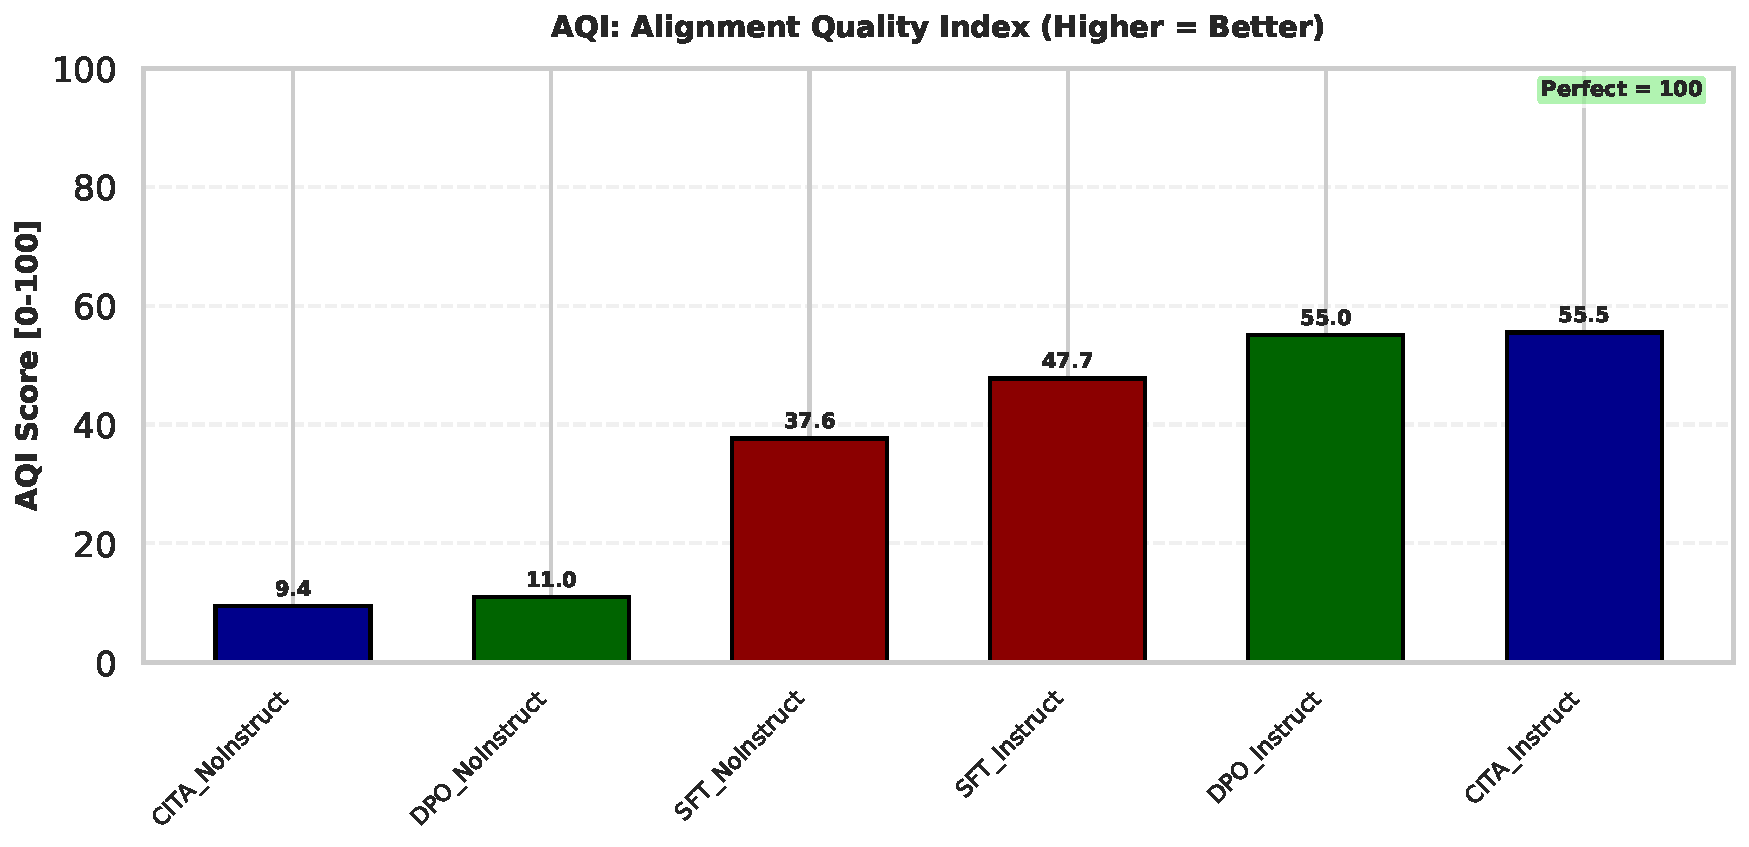
\includegraphics[width=0.85\textwidth]{figures/evaluation/aqi_comparison.pdf}
\caption{\textbf{AQI (Alignment Quality Index)}: CITA\_Instruct (55.5) and DPO\_Instruct (55.0) achieve highest clustering scores. Valid-only scores (hatched) reach 86\%.}
\label{fig:aqi}
\vspace{-3mm}
\end{figure*}

\vspace{-2mm}
\subsection{Combined Analysis}
\label{sec:combined_analysis}

\begin{figure*}[!t]
\centering

\includegraphics[width=0.85\textwidth]{figures/evaluation/combined_plots/radar.pdf}
\caption{\textbf{Instruction Adaptation Radar}: CITA wins 3/5 benchmarks, DPO wins 2/5, SFT wins 0/5. Values show NoInstruct $\rightarrow$ Instruct improvement.}
\label{fig:radar}
\vspace{-3mm}
\end{figure*}

\begin{figure*}[!t]
\centering

\includegraphics[width=0.85\textwidth]{figures/evaluation/combined_plots/heatmap.pdf}
\caption{\textbf{Performance Heatmap}: Original scores with column-normalized colors. Green = best, red = worst per benchmark.}
\label{fig:heatmap}
\vspace{-3mm}
\end{figure*}

\vspace{-2mm}
\subsection{Key Insights}
\label{sec:key_insights}

\paragraph{TruthfulQA is the Differentiator.} On TruthfulQA, CITA improves by +0.054 (becoming appropriately more/less confident when instructed), while DPO shows negligible change (+0.001). This demonstrates CITA's superior ability to \textit{internalize} uncertainty calibration instructions.

\paragraph{CITA Achieves Higher Margins with Lower Accuracy.} Despite similar training accuracy ($\sim$89\%), CITA achieves higher reward margins (7.5 vs. 6.0). This validates that mandatory KL prevents margin collapse while enabling stable behavioral switching.

\paragraph{Instruction-Alignment $\neq$ Instruction-Following.} DPO\_I achieves higher absolute ISD scores, but CITA\_I shows more consistent improvement across diverse benchmarks. This suggests CITA achieves \textit{deeper} instruction-alignment rather than surface-level following.
